\chapter{Introduction to \SB{} and \cocos{} }
Now it's time to dive into 2D Game Development! For this chapter I will assume
that you haven't written a game with a game engine so I will explain the
relevant concepts fairly detailed.

\section{Installing the software}
In general there are two ways to install \cocos{} depending on whether you want
to use \SB{} or not. Throughout this book we will be using \SB{} to set up all
of our projects, therefore we will only install \SB{} which will come bundled
with the latest version of \cocos{}. 

Installing \SB{} is easy, simply open the \textit{App Store} app on your Mac and
search for \textit{SpriteBuilder}:

\begin{figure}[H]
		\centering
		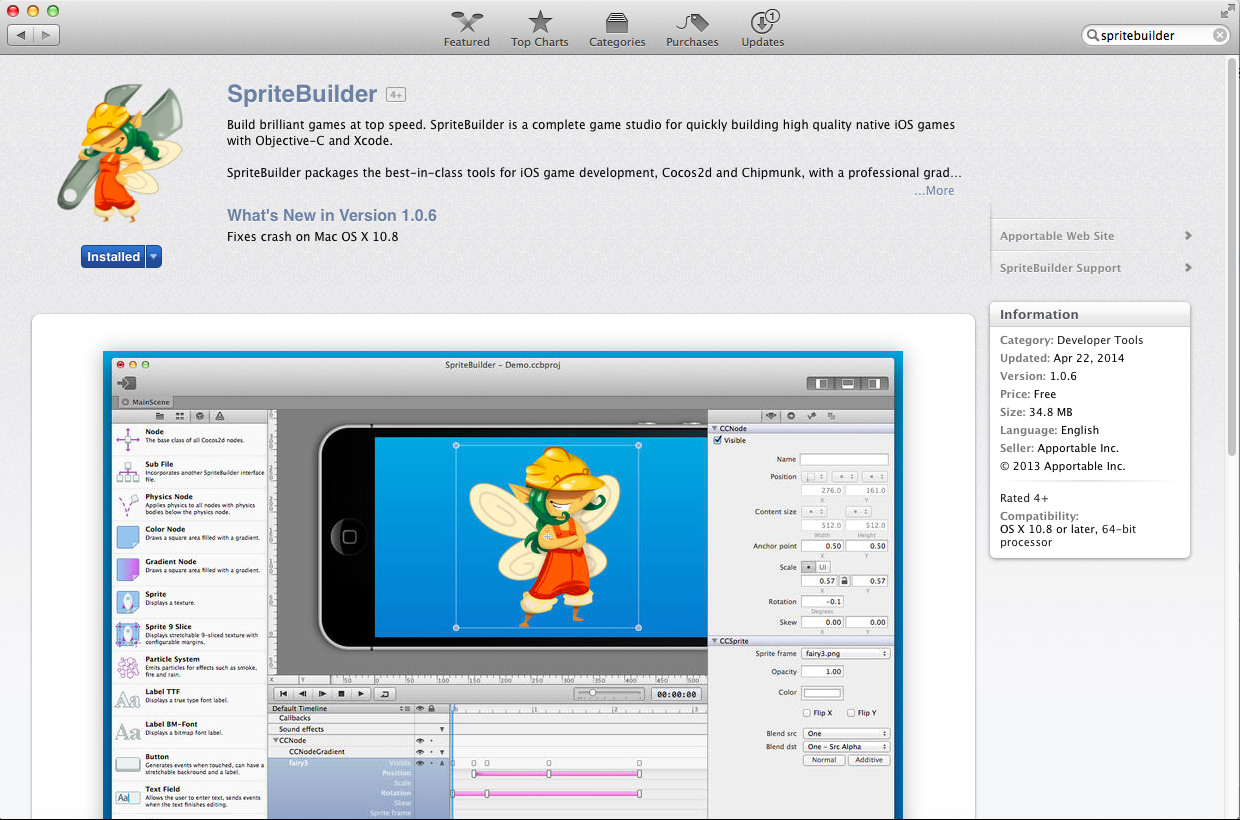
\includegraphics[width=200pt]{images/cocos2d/setup/mac_appstore_install.png}     
		\caption{\cocos{} Technology Stack}
\end{figure}

Well done! Later throughout this chapter you will learn how to set up your first
project!

\section{Introduction to \cocos{}}
To understand what \cocos{} is, it is helpful to look at the history of game
development. The first video games were written in assembler (a very low level
programming language) and images were drawn to the screen by manually setting
colors for certain pixels. Since then a wealth of frameworks and libraries has been written to make the life of a game
developer easier. Throughout this book you will learn how powerful \cocos{} is
and how little code you will need for the basic building blocks of your games.

Here are some of the most important features of \cocos{} that make 2D game
development a lot easier:
\begin{description}
  \item[Structure] like most game engines \cocos{} demands a specific structure
  of the code for your game, making most design decisions simple
  \item[Scene Graph and Sprites] loading an image for a character and adding it
  to the gameplay scene can happen in two lines of code
  \item[Action System] a sophisticated action system allows to define movements
  of objects and animations
  \item[Integrated Physics Engine] automatically calculates movements of
  objects, collisions and more.
\end{description}
There are a whole bunch of more features - but this brief outline shows the most
important ones and should give you an idea why almost all game developers these
days use game engines. 

\cocos{} is built on top of OpenGL ES 2.0. If you have ever written OpenGL code
before you know that it takes many lines of code to draw a textured rectangle on
the screen. \cocos{} abstracts all of these tasks for you, you can go a very
long way without writing any OpenGL code. The following diagram shows which
technologies are used by \cocos{}:

\begin{figure}[H]
		\centering
		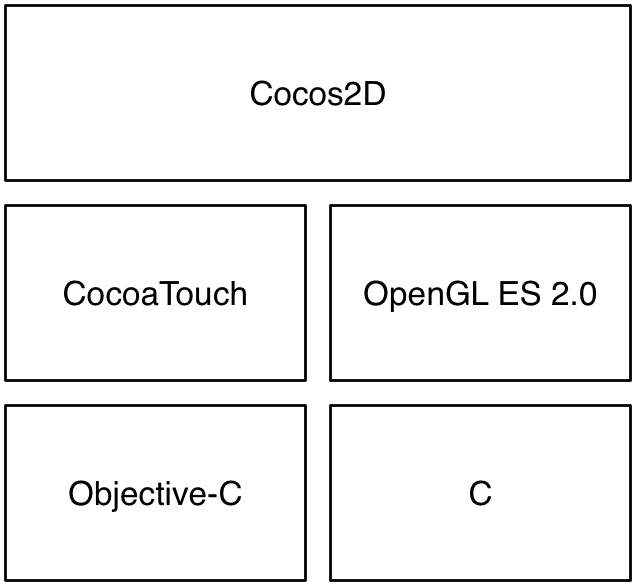
\includegraphics[width=120pt]{images/cocos2d/TechnologyStack.png}     
		\caption{\cocos{} Technology Stack}
\end{figure}

As a \cocos{} developer you define which scenes exist in your game, which
objects are part of these scenes and which size, position and appearance these
objects have and \cocos{} will use OpenGL to render the scene you have
described. In order to provide this functionality \cocos{} consists of many
classes - some important ones will be discussed in this chapter. All \cocos{}
classes use the \textit{CC} prefix (\ccscene{}, \ccnode{}, etc.).

You have probably realized this already - when working with a 2D game engine for
the first time you will be introduced to a whole set of new terminology. Just as a framework to write desktop
applications knows the concept of windows, buttons and mouse clicks a 2D game
engine comes with its own set of terms and techniques. We will spent the next
sections discussing the important terms in detail.

\subsection{Scenes}
For explaining the important terms and concepts of \cocos{} I will use a top
down approach. First we will learn how games that use \cocos{} are structured.
On the highest level of structure we have a concept called \textit{scenes}. By default every scene in
\cocos{} is full-screen. This means for every screen in your game you will use
one scene.

Here's an example from the MakeGamesWithUs game \textit{Deep Sea Fury}:
% add image
You can see that the game consists of the start scene, the gameplay scene and
the game over scene.

A \cocos{} developer creates scenes by using the \ccscene{} class. Another
important \cocos{} class for scene handling is \ccdirector{}. The \ccdirector{}
class is responsible for deciding which scene is currently active in the game
(\cocos{} only allows one active scene at a time). Whenever a developer wants to
display a scene or transition between two scenes he needs to use the
\ccdirector{} class.

This means creating and displaying a new scene is a two step process:
\begin{enumerate}
\item Create a new instance of \ccscene{}
\item Tell the \ccdirector{} to display this new scene
\end{enumerate}

You will learn a lot more about this down the road, but the important bottom
line is: \textit{Scenes are the highest level of structure in your game and a
class called \ccdirector{} decides which scene is currently displayed}.

\subsection{Nodes}
Everything that is visible in your \cocos{} game (and a couple of invisible
objects) are \textit{nodes}. Nodes are used to structure the content of a scene.
Every node can have other nodes as its children. \cocos{} provides a huge amount
of different node types. Every node type is a subclass of \ccnode{}.

Most nodes are used to represent an object on the screen (an image, a solid
color, an UI element, etc.), a few other nodes are only used to group other
nodes. All nodes have a size, positions and children (and many other properties
which are less important for us right now). Here are some of the popular
node types of \cocos{}:

\begin{description}
  \item[CCSprite] represents an image or an animated image. Used for characters,
  enemies, etc.
  \item[CCColorNode] a node being displayed in one plain color.
  \item[CCLabelTTF] a node that can represent text in any TTF font.
  \item[CCButton] a interactive node that can receive touches.
\end{description}

Nodes and their children form a scene graph. The concept of a scene graph isn't
unique to \cocos{} it is a common concept of 2D and 3D graphics. A scene graph
is a hierarchy of many different nodes. 

\subsection{Scene Graphs}
Let's take a look at simple example of a scene graph:

\begin{figure}[H]
		\centering
		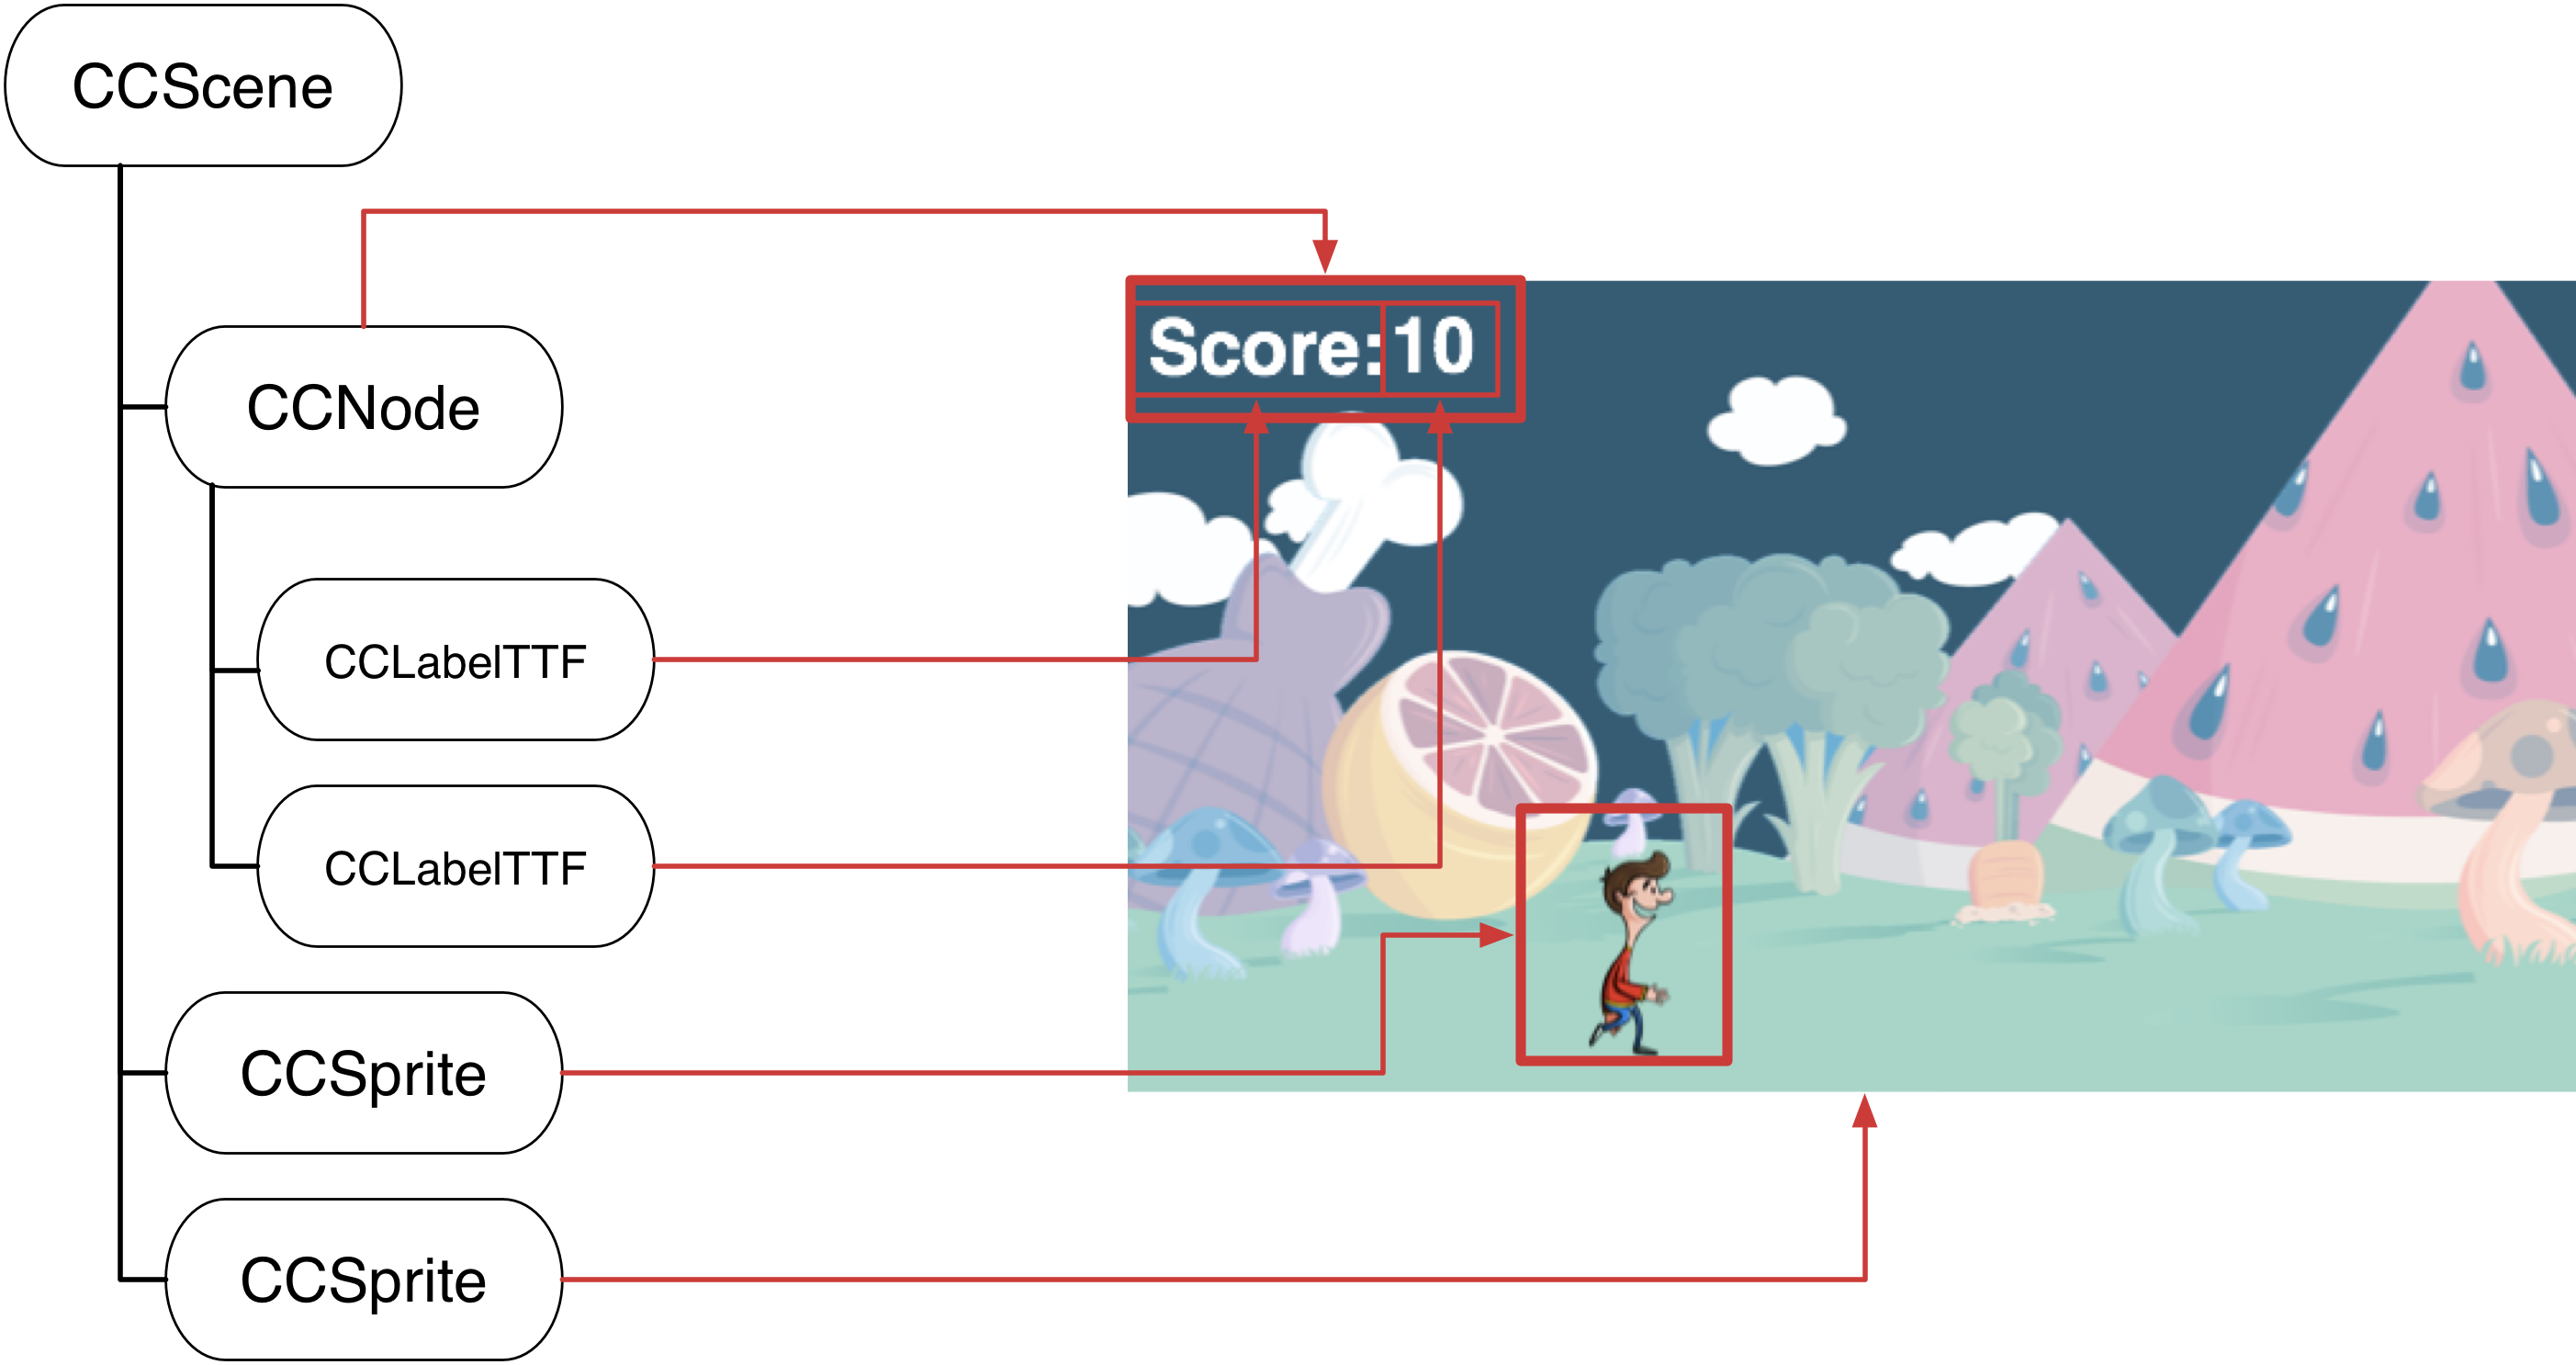
\includegraphics[width=290pt]{images/cocos2d/SceneGraph.png}     
		\caption{\cocos{} Scene Graph}
\end{figure}

On the left side of the image you can see the node hierarchy. On the first level
you have the \ccscene{}. Then we have a \ccnode{} with to children of type
\cclabel{}. This \ccnode{} is the first example of a grouping node. Instances of
\ccnode{} don't have any appearance they are solely used to group other nodes.
Throughout this book you will learn that it often makes sense to group nodes
under certain parent nodes. The main reason is that all children are placed
\textit{relative} to their parents. So if we would want to move the scoreboard
of the example above to the top right corner we would only have to move the
parent node instead of both child nodes. As you can imagine this becomes
even more relevant in games that have ten or more entries in their scoreboard.

\begin{bestpractice}[frametitle={Structuring Nodes}] 
Always group nodes that logically belong together under one parent node. That
will save you a lot of time when you change the layout of your scene.
\end{bestpractice}

The other two objects in the scene graph are simpler. One represents the
background image the other one the main character.

For some games scene graphs can get very complex and include hundreds of
different nodes. The key takeaways for now are:

\begin{enumerate}
  \item Every node in \cocos{} can have children
  \item A hierarchy of nodes is called a scene graph
  \item Children of nodes are placed relative to their parents - often it is
  useful to group nodes that are moved together under one parent
\end{enumerate}

Now that you have a basic understanding of how games are structured in \cocos{}
we will take a look at a second tool which we will be using throughout this
book: \SB{}.

\section{Introduction to \SB{}}
You have learned the fundamentals of the game engine we will use. Now we will
take a look at a tool called \SB{} which we will use to create the majority of
our game content. The main purpose of \SB{} is to provide a visual editor for
the creation of scenes, animations and more. For most games you will create some
basic mechanics in code (enemy movement, score mechanism, etc.) but you will create
the most of your game content in \SB{} since it is a lot easier to create
levels, menus and other scenes in an editor that provides you with a live
preview instead of putting these scenes together in code.

\subsection{Creating a first project}
To dive into the features of \SB{} we will create our first project! 
Create a new project by opening SpriteBuilder and selecting \textit{File > New >
Project...}:
\begin{figure}[H]
		\centering
		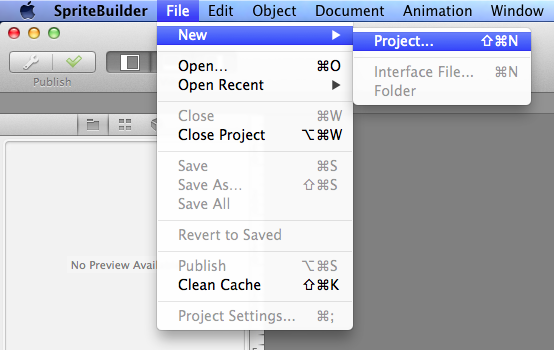
\includegraphics[width=290pt]{images/cocos2d/setup/spritebuilder_new_project.png}     
\end{figure}

\SB{} will ask for a name and a location for the new project. Name it
\textit{HelloSB}. After you create the project the folder structure should look similar to this:
\begin{figure}[H]
		\centering
		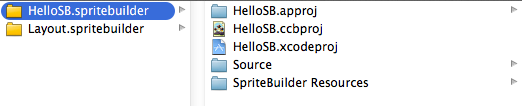
\includegraphics[width=250pt]{images/cocos2d/setup/project_structure.png}     
		\caption{\SB{} project folder structure}
\end{figure}

Every \SB{} project is contained in a \textit{.spritebuilder} folder. Within
this folder all the files of the \SB{} project are stored - along with an \xcode{}
project. 

\begin{lamp}[frametitle={\SB{} and Xcode}] 
\SB{} will create an \xcode{} project for every new project you create! The
\xcode{} project will automatically contain the newest version of \cocos{} -
very handy.
\end{lamp}

Later on you will learn more about how the \SB{} project and the \xcode{}
project work together. The general rule is that all code will be part of the
\xcode{} project and most content creation will happen in the \SB{} project.

\subsection{The Editor}
When you have created your first \SB{} project you will see that the \SB{} UI
gets enabled. Let's take a look at the different parts of the editor to get a
better understanding of \SB{}.

The \SB{} interface is divided into 4 main sections:
\begin{figure}[H]
		\centering
		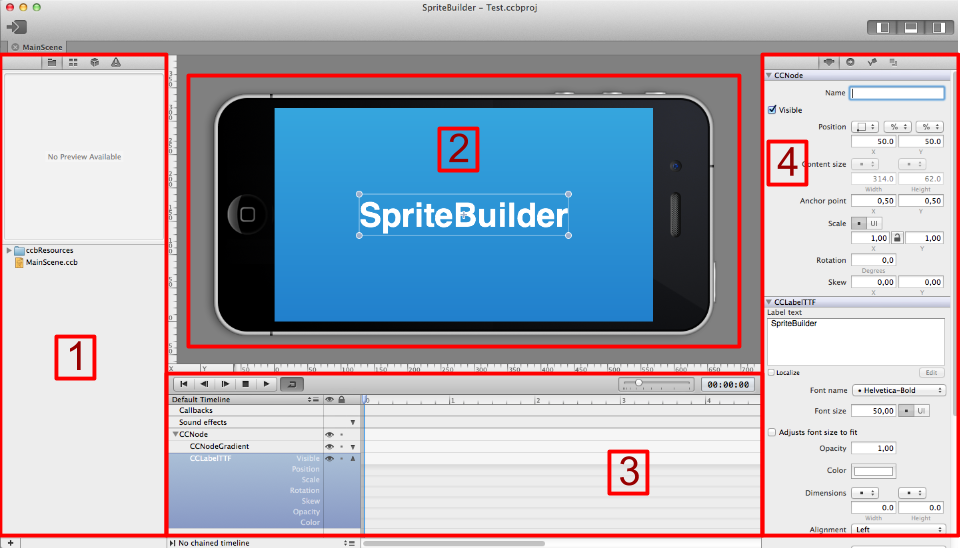
\includegraphics[width=290pt]{images/spritebuilder/spritebuilder_ui.png}     
\end{figure} 
\begin{enumerate}
  \item \textit{Resource/Component Browser:} Here you can see the different
  resources and scenes you have created or added to your project. You can also select different types of Nodes and drag them into your scene.
  \item \textit{Stage:} The stage will preview your current scene. Here you can
  arrange all of the Nodes that belong to a scene. 
  \item \textit{Timeline:} The timeline is used to create animations within
  SpriteBuilder.
  \item \textit{Detail View:} Once you select a node in your scene, this detail
  view will display a lot of editable information about that node. You can modify positions, content (the text of a label, for example) and physics properties.
\end{enumerate}
Let's take a closer look at some of the most important views.

\subsubsection{File View}
The first tab in the resource/component browser represents the \textit{File
View}.
It lists all the \textit{.ccb} files and resources that are part of the \SB{}
project:
\begin{figure}[H]
		\centering
		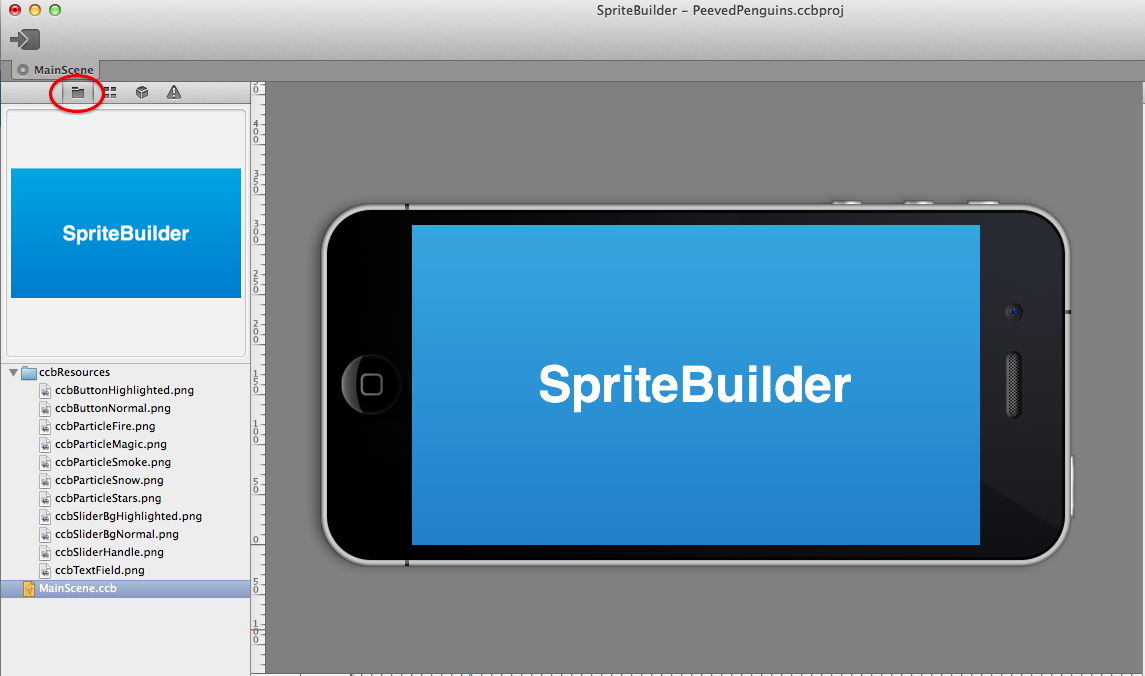
\includegraphics[width=290pt]{images/spritebuilder/spritebuilder_fileview.png}     
\end{figure} 
In this view you can add new resources and restructure your project's folder
hierarchy.
\subsubsection{Node Library}
The third tab in the left view is the {Node Library}:
\begin{figure}[H]
		\centering
		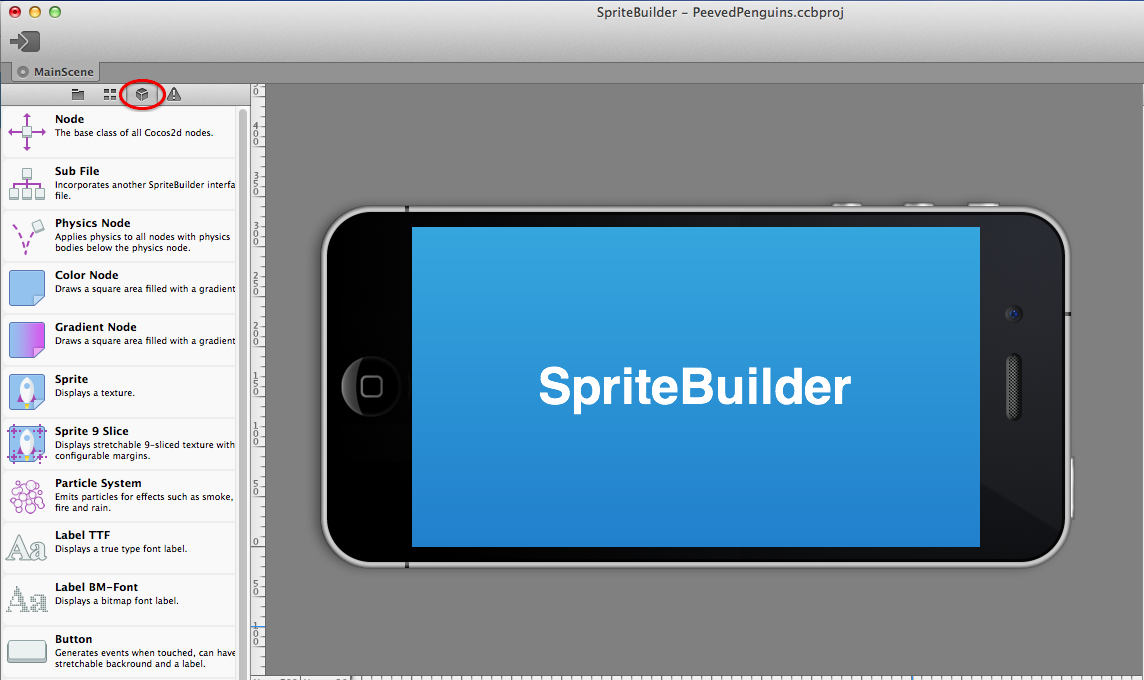
\includegraphics[width=290pt]{images/spritebuilder/spritebuilder_nodeview.png}     
\end{figure} 
This panel shows you all available node types you can use to construct your
gameplay scenes and menus. You will drag these nodes from this view to the stage
in the center to add them to your scenes.

\subsubsection{Inspector}
The first tab of the Detail View (the right panel) is
the Inspector. Once you have selected an object on your stage you can use this panel to modify many of its properties, like position and color:
\begin{figure}[H]
		\centering
		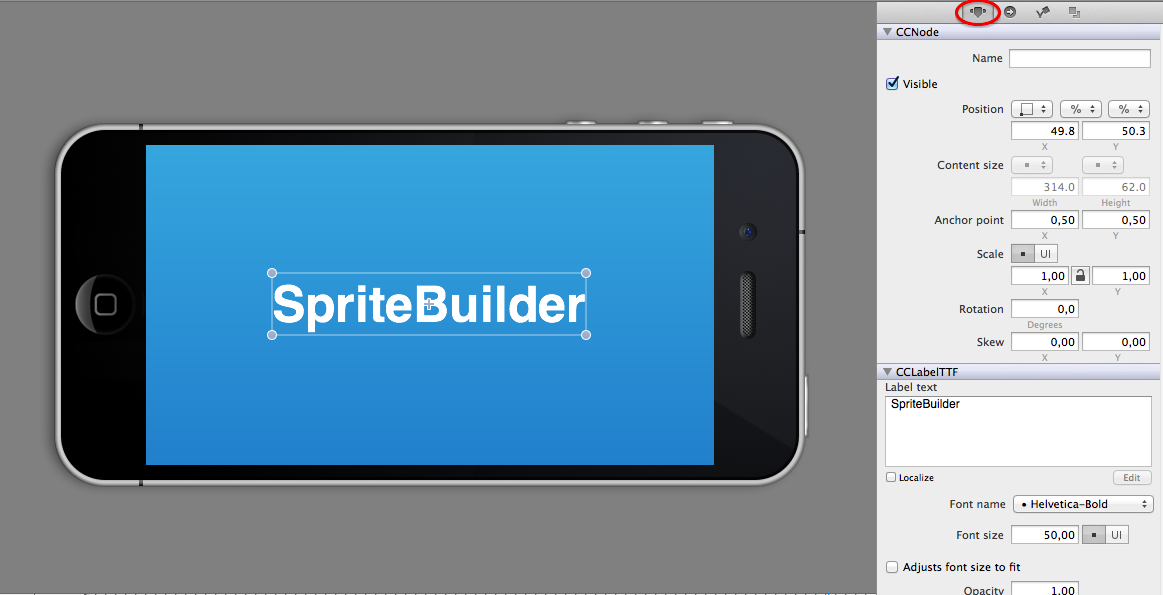
\includegraphics[width=290pt]{images/spritebuilder/spritebuilder_inspector.png}     
\end{figure} 

\subsubsection{Code Connections}
The second tab on the right panel let's you manage code connections for your
selected node. As mentioned previously the entire code for your games will be
written as part of the \xcode{} project. This view allows you to create
connections between the \xcode{} project and the \SB{} project. For example you can set a custom Objective-C class for a node or you can select
a method in your code that shall be called once a button in your scene is tapped. 

\begin{figure}[H]
		\centering
		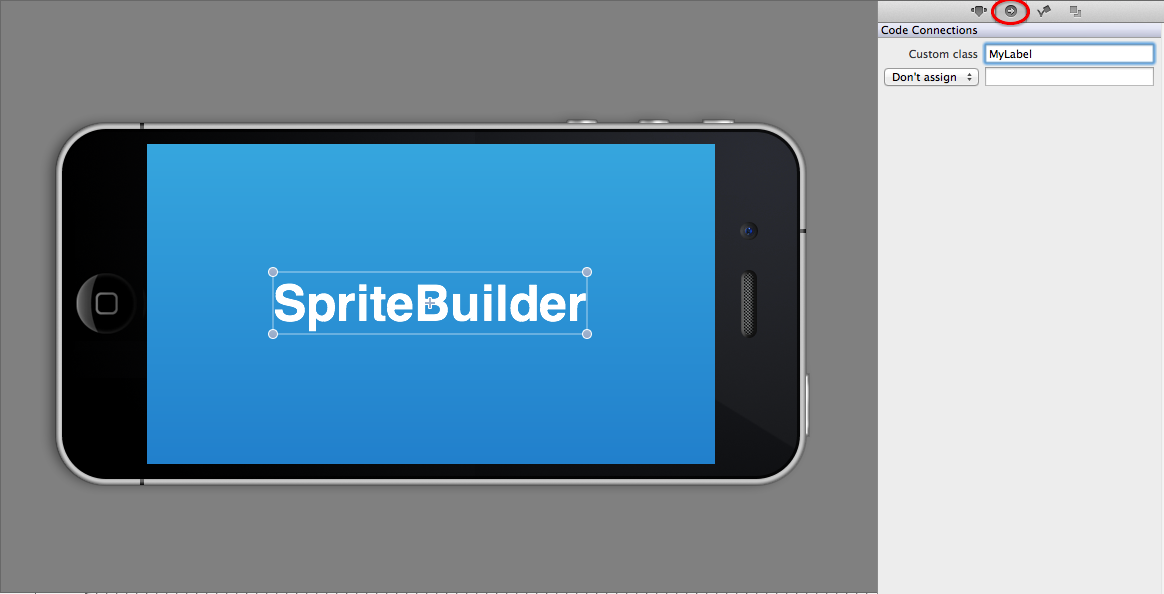
\includegraphics[width=290pt]{images/spritebuilder/spritebuilder_codeconnections.png}     
\end{figure} 
Code connections will be discussed in detail later on.

\subsection{\ccbfile{}s}
\ccbfile{}s are the basic building blocks of your \SB{} project. Every scene in
your game that is created with \SB{} is represented by one \ccbfile{}. However
\ccbfile{}s are not only used to create entire scenes - they are used to create
any kind of scene graph. \SB{} provides different kinds of templates depending
on which type of scene graph you want to create. You get an overview of the
available \ccbfile{} templates when you create a new one, by selecting
\textit{New > File... } from the \textit{File} menu in \SB{}:
\begin{figure}[H]
		\centering
		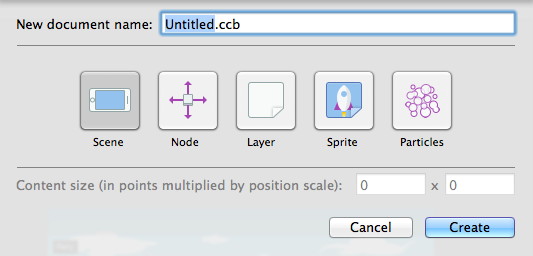
\includegraphics[width=240pt]{images/spritebuilder/new-ccb.png}     
\end{figure} 
These are the different templates briefly explained:
\begin{description}
\item[Scenes] will fill the full screen size of the device.
\item[Nodes] used primarily for grouping functionality, don't have a size.
\item[Layers] are nodes with a content size. This is useful, for instance, when
creating levels or contents for scroll views.
\item[Sprites] used to create (animated) characters, enemies, etc.
\item[Particles] is used to design particle effects.
\end{description}
You will get a good understanding when to use which type of \ccbfile{} once we
get started with our example projects. The key takeaway is that \ccbfile{}s are
used by \SB{} to store an entire scene graph including size, positions and many
other properties of all the nodes that you have added.

\subsection{How \SB{} and \xcode{} work together}
I have mentioned how \SB{} and \xcode{} integrate a couple of times briefly. In
order to be a well versed and efficient \SB{} game developer it is very
important to understand the details of this cooperation.

When creating a \SB{} project, \SB{} will create and maintain a corresponding
\xcode{} project. In \SB{} will you create multiple \ccbfile{}s that describe
the content of the scenes in your game. You will also add the resources that
you want to use in your game and set up code connections to interact with the
code in your \xcode{} project. \xcode{} will be the place where you add code to
your project and where you run the actual game.

Since \xcode{} is the tool that actually compiles and runs your game it needs
to know about all the scenes and resources that are part of your \SB{} project.
Therefore \SB{} has a \textbf{publish} functionality, provided by a button in
the top left corner of the interface:
\begin{figure}[H]
		\centering
		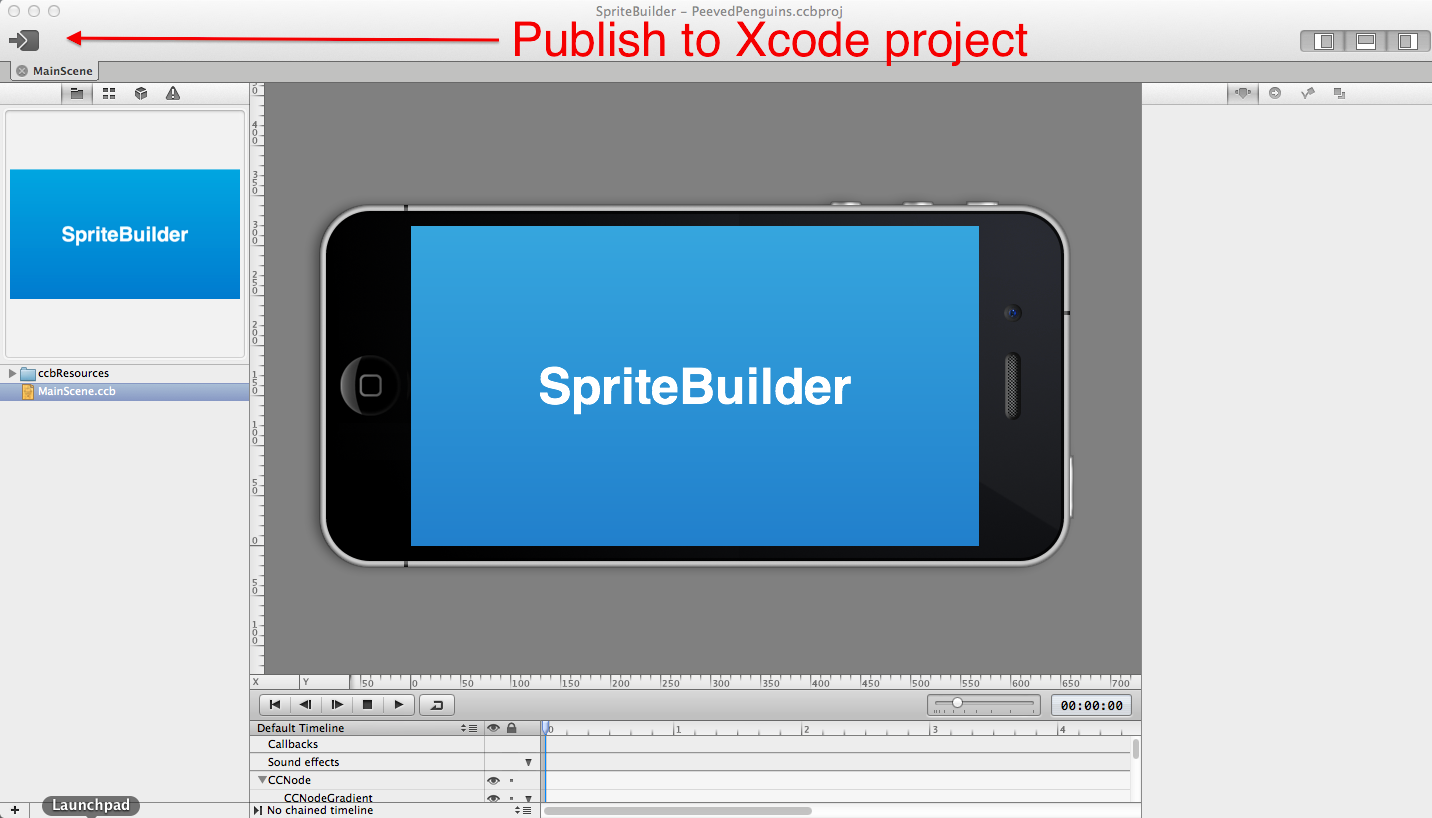
\includegraphics[width=290pt]{images/spritebuilder/spritebuilder_publish_button.png}
		\caption{Use the publish button to update your \xcode{} project with the
		latest changes in your \SB{} project.}
		%\label{labelstruct} 
\end{figure}
Using that button, you publish your changes in your
\SB{} project to your \xcode{} project. Whenever you changed your \SB{}
project and want to run it you should hit this button before building the \xcode{}
project.

Here's a diagram that visualizes how \SB{} and \xcode{} work together:
\begin{figure}[H]
		\centering
		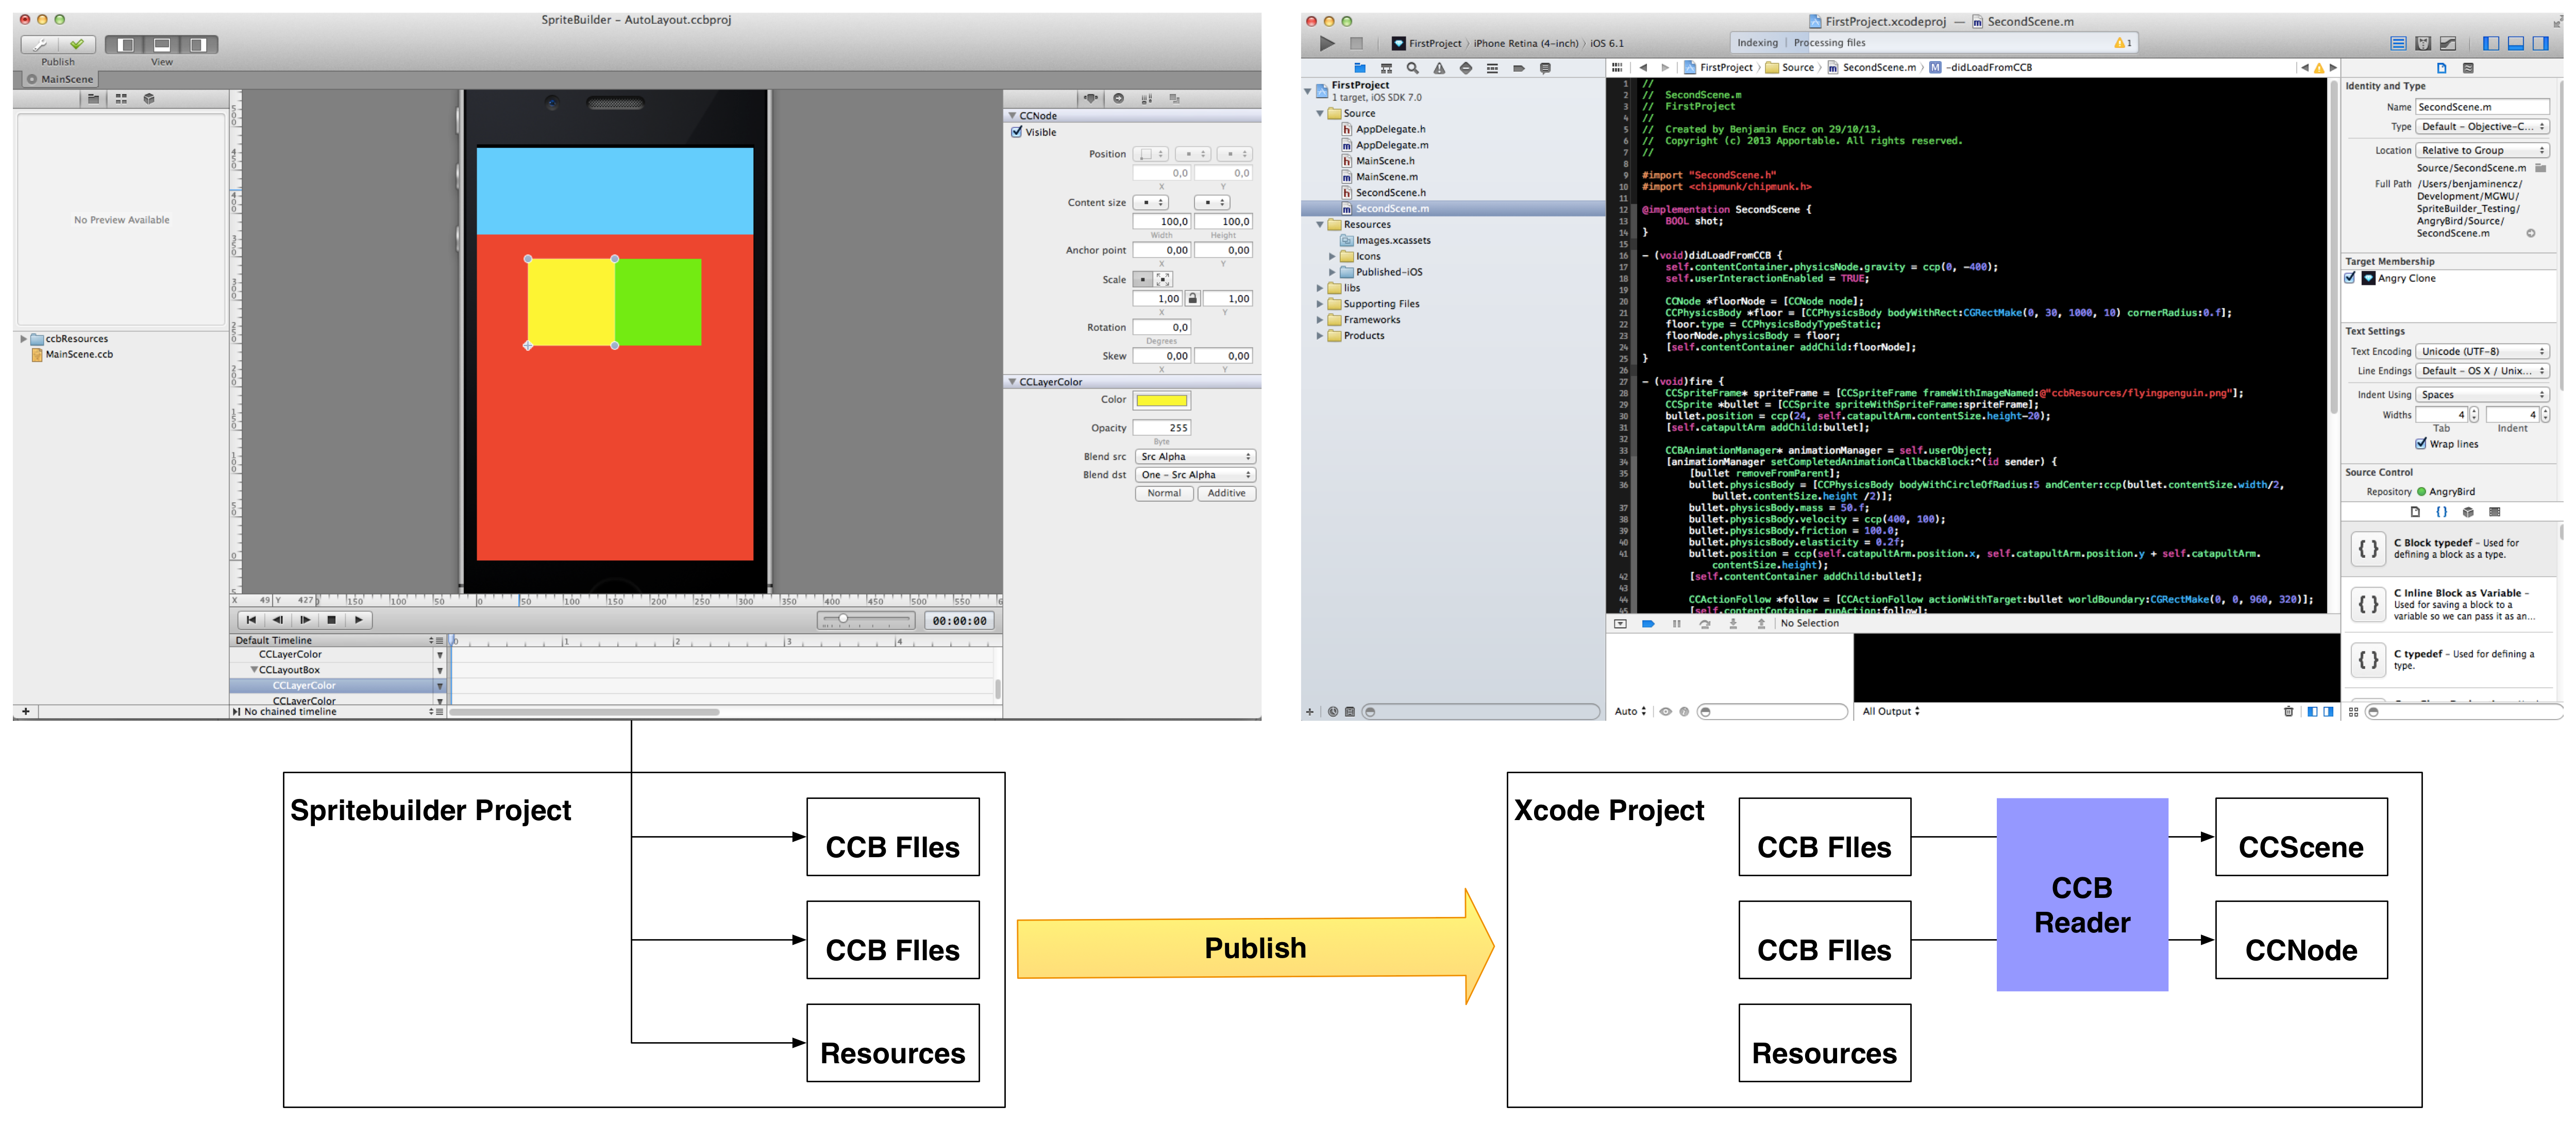
\includegraphics[width=290pt]{images/spritebuilder/spritebuilder_publishing.png}
		\caption{\SB{} creates and organizes a \xcode{} project for you. Adding
		all the resources and scenes you have created.}
		%\label{labelstruct} 
\end{figure}
\ccbfile{}s created in \SB{} store a scene graph; the hierarchy and positions of
your nodes. When publishing a \SB{} project the \ccbfile{}s and all other
project resources are copied to your \xcode{} project.
When running the project in \xcode{} a class called CCBReader will parse your
\ccbfile{}s and create the according \ccnode{} subclasses to reconstruct the scene
graph you have designed in \spriteb{}.

If you would use \cocos{} without \SB{} you would manually create instances of
\ccnode{}, \ccsprite{}, etc. in code and add children to these nodes -
essentially building the entire scene graph in code.

When using \SB{} the CCBReader class will build this scene graph for you, based
on the information stored in the \ccbfile{}s that you created in \SB{}.

Another important part of information contained in \ccbfile{}s that we have not
discussed in detail yet are \textit{Code Connections}.

\subsection{Code Connections}
Code connections are used to create links between your scenes in \SB{} and your
code in \xcode{}. There are three basic types of code connections:
\begin{description}
\item[Custom Classes] are an important information for the CCBReader. As
mentioned previously the CCBReader builds the scene graph by creating different
nodes based on the information in your \ccbfile{}. By default it will create an
instance of \ccsprite{} for every sprite you added in \SB{} an instance of \ccnode{} for every node you added, etc. Often
however you will want to add custom behaviour to a node (for example a movement
pattern for an enemy). Then you will have to use the \textit{Custom Class}
property to tell the CCBReader which class it should instantiate instead of the
default one. Whichever class you enter here needs to be a subclass of the
default class (e.g. a subclass of \ccsprite{}). You will learn how to use this
feature in the final project of this chapter!
\item[Variable Assignments] If you have assigned a \textit{Custom Class} you can
use variables assignments to retrieve references to different nodes in the
scene. For example a character might want a reference to its right arm node (a
child of the character node) in order to move it. 
\item[Callbacks] are only available to UI elements like buttons and sliders.
They allow you to decide which method should be called on which class once a
button is pressed.
\end{description}
Now you should have an idea about what code connections are used for and which
kinds exist. We will discuss the details of all types when we use them as part
of our example projects.

\section{A first \SB{} project} 
You have already created the \SB{} project called \textit{HelloSB}. Now we will
start adding some content to it. The project built in this chapter will consist
of two scenes one start screen and one game screen. In the game screen the user will be able to spawn randomly
colored squares by tapping on the screen.
\begin{figure}[H]
		\centering
		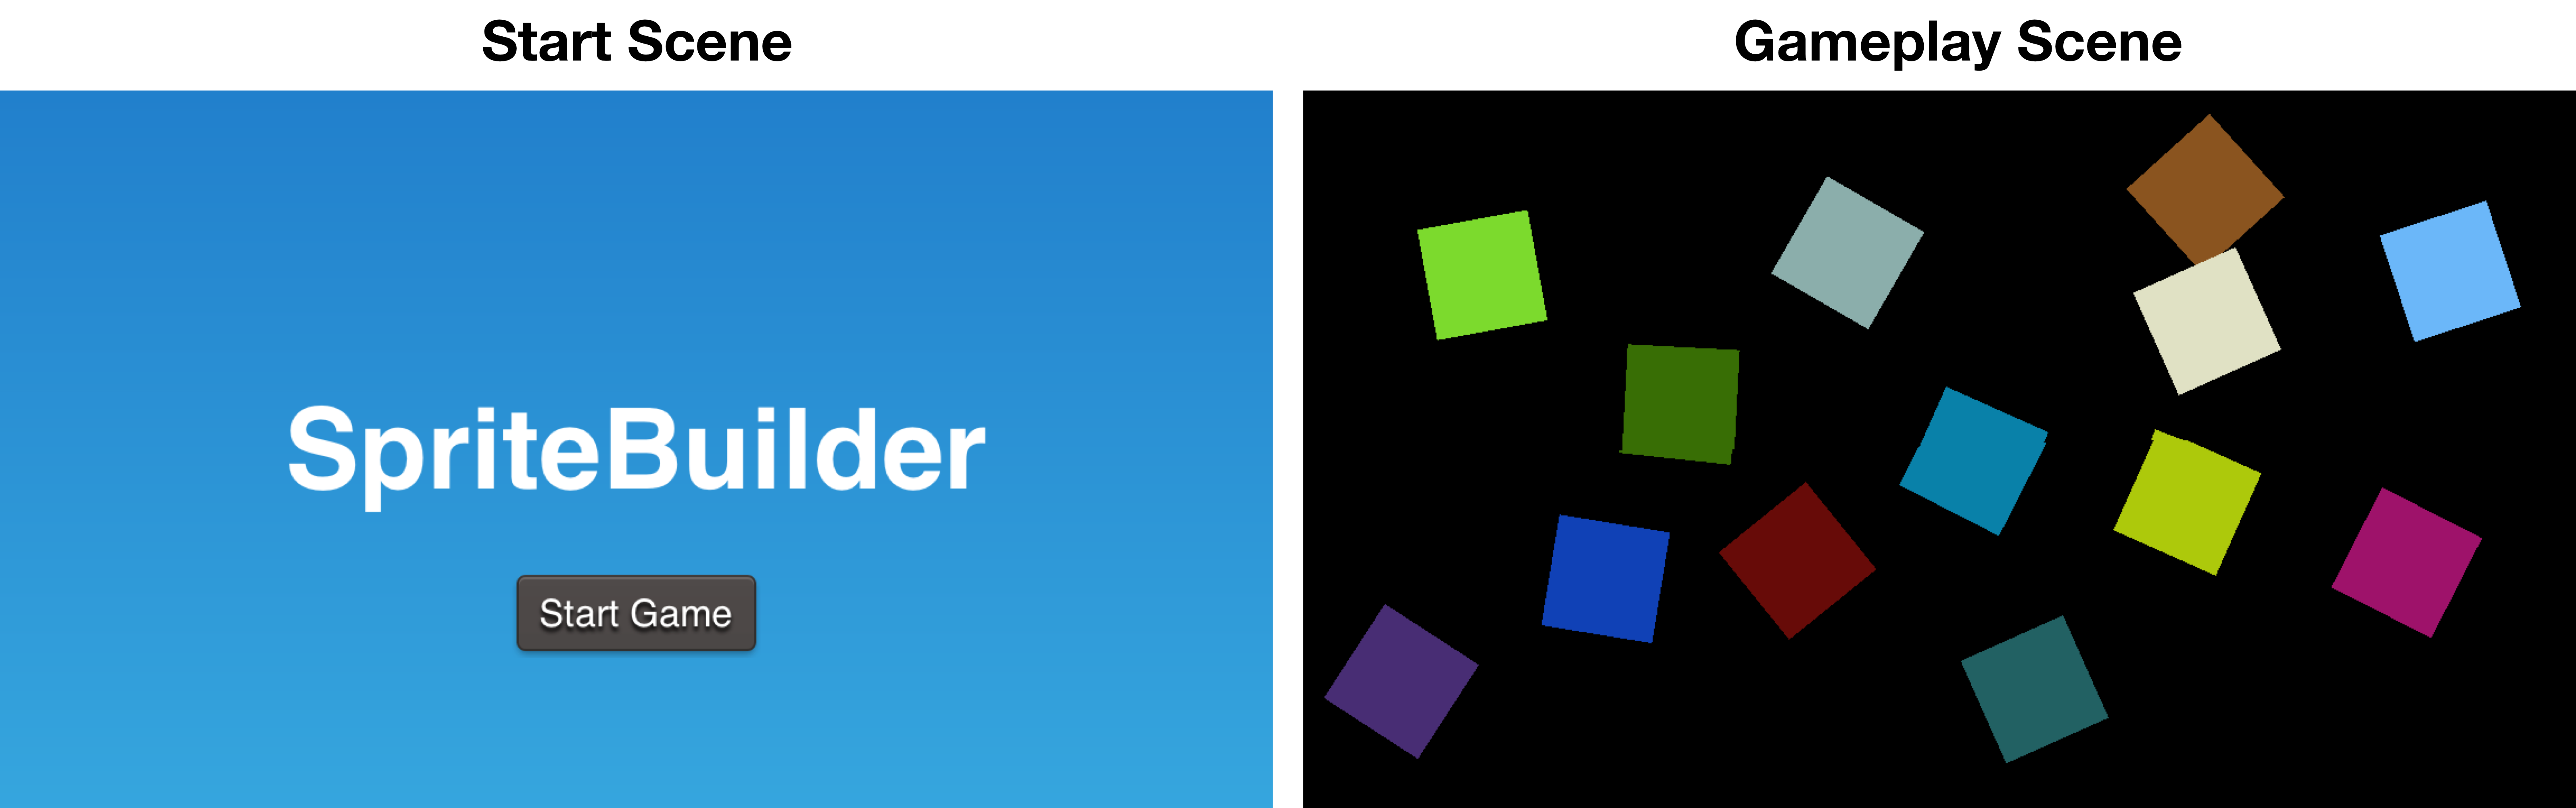
\includegraphics[width=290pt]{images/firstproject/first_project.png}
		\caption{The project build throughout this chapter}
		%\label{labelstruct} 
\end{figure}
By creating this project you will learn all of the following:
\begin{itemize}
  \item Creating scenes in \SB{}
  \item Creating code connections (callbacks, variable assignments and custom
  classes)
  \item Switching between different scenes
  \item Manipulate a scene graph from code (add/remove nodes, load CCB Files and
  add them to the scene)
  \item Use the \cocos{} action system to create animations
  \item Use the \cocos{} touch handling system to capture touches
\end{itemize}

\subsection{Setting up the first scene}
%explain code connections in detail here
Now it is time to open the \textit{HelloSB} \SB{} project. We want to add a
\textit{Start Button} to the first scene. When this button is tapped we want to
switch to the second scene. Start by adding a button to the first scene:

\begin{figure}[H]
		\centering
		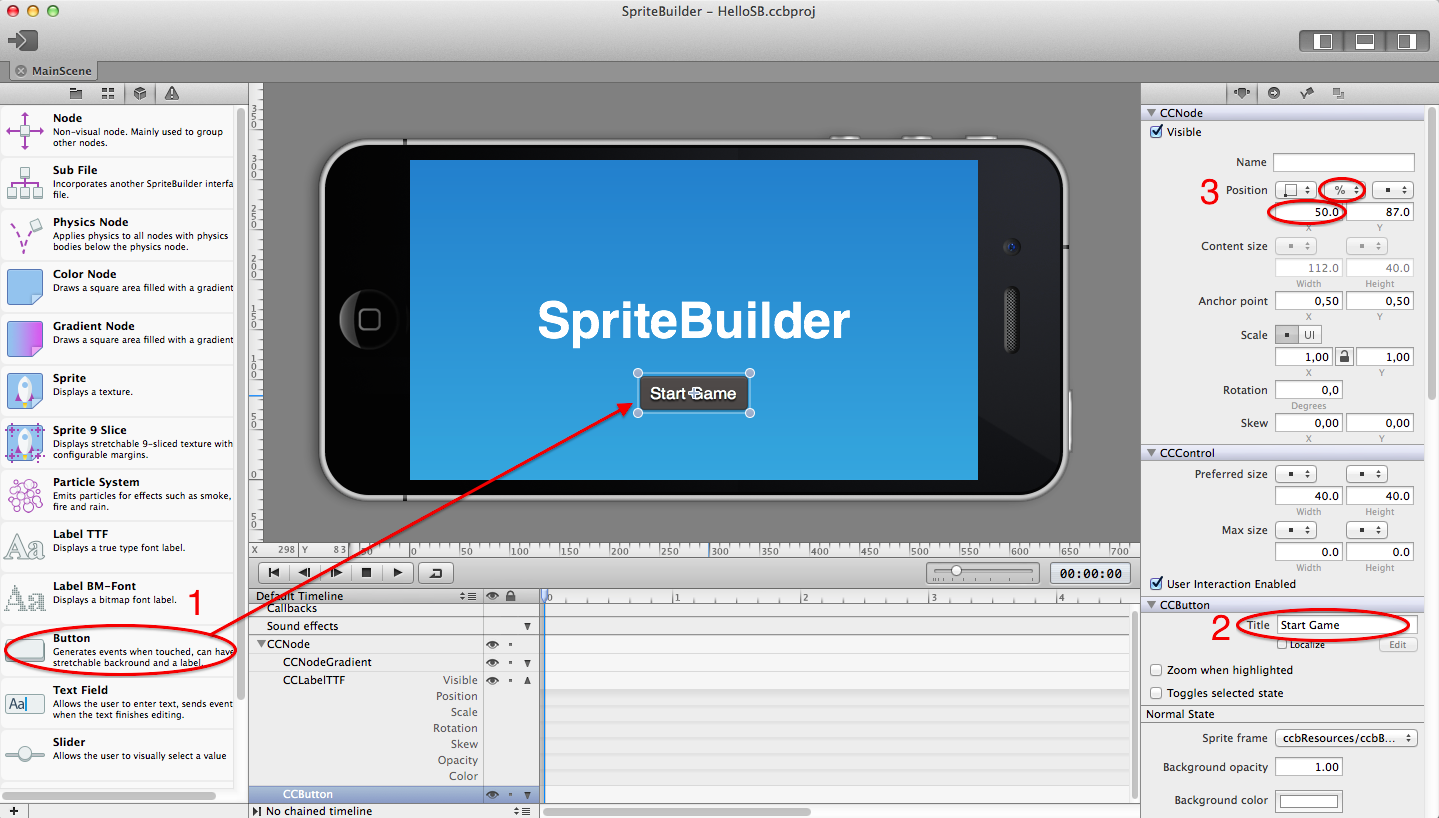
\includegraphics[width=300pt]{images/firstproject/add_button.png}
		\caption{The project build throughout this chapter}
		%\label{labelstruct} 
\end{figure}

One simple button, but since this is your first action in \SB{} there's
\textit{lots} to explain about it. Let's look at the three steps highlighted in
the image above, step by step.

\begin{description}
\item[(1)] Open \textit{MainScene.ccb} by double clicking it in the left
resource pane. Then open the third tab in the left pane, the \textit{Node
Library}. Remember, this section shows you all the different node types
supported by \SB{}. Select the \textit{Button} and drag it over to the stage,
dropping it below the existing label. Dropping it on the stage will add this
node to your scene. Another way of adding a node to a scene is dropping it to
the timeline at the bottom of the screen - we will look at this later.
\item[(2)] Make sure the button is selected, because we want to change some
properties of it. Whenever you have selected a node the right pane will display
all the properties you can edit. Navigate to the \textit{Title} textfield in the
property pane and change the title of the button to \textit{Start Game}.
\item[(3)] So far - so simple. Step number three will expose you to a very
interesting feature of \SB{}: the positioning system. 
\end{description}

\begin{details}[frametitle={Positioning System in \cocos{} and \SB{}}] 
The positioning system in \cocos{} is designed from the ground up to make it
easy to design scenes and user interfaces for different screen sizes and
resolutions. The comfortable days where the 3.5-inch iPhone was the only 
available iOS device and defining layouts with absolute positions was acceptable
are finally over. Today app and game developers face a variety of different
devices and customers justifiably expect your software to work great on all of
them. \cocos{} offers the following properties on \ccnode{}s to allow developers
to design their interfaces with great flexibility:

\begin{itemize}
  \item Anchor Point
  \item Reference Corner
  \item Position Type
  \item Size Type
\end{itemize}

\end{details}

